\chapter{Tensorflow基础}
\section{Tensorflow基础概念}
Tensorflow正如它的名字表达的是定义tensor的计算。一个tensor是一个概括的矩阵和向量,并且有能力表示更高的维度,我们写Tensorflow程序,主要的对象就是tf.Tensor,一个tensor定义计算的一部分最后生成值。TensorFlow程序首先用tensor建立一个图,然后运行图获得想要的数据。一个tensor需要指定两个参数:数据类型和形状。Tensor中的数据类型相同,而且总是可知的,形状可能仅仅部分知道。
下面是一些特殊的Tensor类型:
\begin{itemize}
\item	tf.Variable
\item	tf.Constant
\item	tf.Placeholder
\item	tf.SparseTensor
\end{itemize}
\subsection{Rank}
tf.Tensor的rank是对象的维度。TensorFlow的rank和数学中矩阵的rank不一样,下面显示TensorFlow rank和相对应的数学实体
\begin{center}
\begin{tabular}{|c|c|}
\hline
rank&数学实体\\
\hline
0&Scalar(只有值)\\
\hline
1&Vecor(值和方向)\\
\hline
2&矩阵(数值表)\\
\hline
3&3-Tensor\\
\hline
n&n-Tensor\\
\hline
\end{tabular}
\end{center}
\textbf{Rank0}

下面片段展示创建一些0维的变量。
\begin{python}
mammal = tf.Variable("Elephant", tf.string)
ignition = tf.Variable(451, tf.int16)
floating = tf.Variable(3.14159265359, tf.float64)
its_complicated = tf.Variable((12.3, -4.85), tf.complex64)
\end{python}
\textbf{Rank1}
传递列表作为初始值创建1维tf.Tensor对象
\begin{python}
mystr = tf.Variable(["Hello"], tf.string)
cool_numbers  = tf.Variable([3.14159, 2.71828], tf.float32)
first_primes = tf.Variable([2, 3, 5, 7, 11], tf.int32)
its_very_complicated = tf.Variable([(12.3, -4.85), (7.5, -6.23)], tf.complex64)
\end{python}
\textbf{更高的rank:}
二维的Tensor至少有一行一列
\begin{python}
mymat = tf.Variable([[7],[11]], tf.int16)
myxor = tf.Variable([[False, True],[True, False]], tf.bool)
linear_squares = tf.Variable([[4], [9], [16], [25]], tf.int32)
squarish_squares = tf.Variable([ [4, 9], [16, 25] ], tf.int32)
rank_of_squares = tf.rank(squarish_squares)
mymatC = tf.Variable([[7],[11]], tf.int32)
\end{python}
更高rank的Tensor,有n维数组。例如在图像处理,一些tensor的rank为4,维度通常是example-in-batch,image width,image height,color chennel。
\begin{python}
my_image = tf.zeros([10, 299, 299, 3])  # batch x height x width x color
\end{python}
\subsection{获取Tensor对象的rank}
你可以使用tf.rank方法获取tensor对象的rank。例如下面获取my3d的rank。
\begin{python}
r = tf.rank(my2d)#在图运行后,r将保持值3。
\end{python}
\subsection{Tensor的切片}
因为tf.Tensor是n维cell阵列,为了访问tf.Tensor的单个cell,你需要指定索引。
对于rank为0的tensor,不需要索引,因为它已经是单个值了。\par
对于rank1(向量),传递一个索引允许你访问:
\begin{python}
my_scale = my_vector[2]
\end{python}
如果你想动态的选择向量中的元素,你可以指定[]一个tf.Tensor。
传递一个数值访问矩阵的子向量:
\begin{python}
my_row_vetor = my_matrix[2]
my_column_vector = my_matrix[:, 3]
\end{python}
\subsection{形状}
shape是tensor每一维元素的个数。TensorFlow在构造图的时候自动计算形状。有时候自动计算可能不知道rank,如果rank已经知道,每一维的形状可能直到可能不知道。
\begin{tabular}{|c|c|c|c|}
\hline
rank&shape&维数&example\\
\hline
0&[ ]&0-D&O维Tensor,标量\\
\hline
1&[D0]&1-D&一维tensor的形状\\
\hline
2&[D0,D1]&2-D&二维Tensoe的形状\\
\hline
3&[D0,D1,D2]&3-D&三维Tensor的形状\\
\hline
n&[D0,D1,\ldots,$D_{n-1}$]&N维tensor的形状[$D_0,D_1,\ldots,D_{n-1}$]&\\
\hline
\end{tabular}
\subsection{获取tf.Tensor对象的形状}
当建立图的时候tensor的形状已知是很有用的,你可以通过tensor的shape属性得到。得到完全定义的tf.Tensor的形状可以使用Tf.shape操作。这个方法你可以建立一个图操作tensor的形状。

例如,这里是如何如何创建一个和给定矩阵列数相同的全零向量。
\begin{python}
zeros = tf.zeros(tf.shape(my_matrix)[1])
\end{python}
\subsection{改变Tensor的形状}
tensor的元素个数是所有形状值的乘积。标量的元素总是1.因此,因为有相同元素不同形状的tensor,转变它们的形状是很方便的。可以使用tf.reshape.

下面例子展示了如何reshape tensor。
\begin{python}
rank_three_tensor = tf.ones([3, 4, 5])
matrix = tf.reshape(rank_three_tensor, [6, 10])  # Reshape existing content into
                                                 # a 6x10 matrix
matrixB = tf.reshape(matrix, [3, -1])  #  Reshape existing content into a 3x20
                                       # matrix. -1 tells reshape to calculate
                                       # the size of this dimension.
matrixAlt = tf.reshape(matrixB, [4, 3, -1])  # Reshape existing content into a
                                             #4x3x5 tensor

# Note that the number of elements of the reshaped Tensors has to match the
# original number of elements. Therefore, the following example generates an
# error because no possible value for the last dimension will match the number
# of elements.
yet_another = tf.reshape(matrixAlt, [13, 2, -1])  # ERROR!
\end{python}
\subsection{数据类型}
tf.Tensor不可能有一个以上的数据类型。然而序列化数据结构作为字符串尺寸处在tf.Tensor里是可能的。

可以使用tf.cast转换一种数据类型到另一种。
\begin{python}
# Cast a constant integer tensor into floating point.
	float_tensor = tf.cast(tf.constant([1, 2, 3]), dtype=tf.float32)
\end{python}
通过Tensor的dtype查看tensor的数据类型。你通过python对象创建tf.Tensor的时候需要指定数据类型。如果你不指定TensorFlow选择一个代表你数据的数据类型。TensorFlow转换Python整数为tf.int32,浮点数为tf.float32。转换数组时TensorFlow用和numpy相同的规则。
\subsection{计算Tensor}
当计算图被创建后你可以通过运行计算tf.Tensor获取指定的值。用Tensor.eval方法简单的计算:
\begin{python}
constant = tf.constant([1,2,3])
tensor = constant*constant
print(tensor.eval())
\end{python}
eval方法仅仅当tf.Session()被激活时可用。Tensor.eval然后会得到一个和tensor相同内容的numpy数组。有时候没有上下文计算tf.Tensor是不可能的。例如,tensor依赖于Placeholder在提供给Placeholder值之前不能计算。
\begin{python}
p = tf.placeholder(tf.float32)
t = p + 1.0
t.eval()  # This will fail, since the placeholder did not get a value.
t.eval(feed_dict={p:2.0})  # This will succeed because we're feeding a value
                           # to the placeholder.
\end{python}
其它的模型结构在计算tf.Tensor时可能很复杂。TensorFlow不能直接计算定义在函数内部的或者控制流结构的tf.Tensor。如果tf.Tensor依赖于队列中的值,计算tf.Tensor仅仅入队的时候工作,负责计算被挂起。当和queue工作的时候,记得在计算任何tf.Tensor之前用tf.train.start\_queue\_runners。
\subsection{打印Tensor}
出于调试目的,你想要打印tf.Tesor的值。tfdbg提供了高级的调制支持。TensorFlow用下面的模板打印tf.Tensor:
\begin{lstlisting}[language=Python]
t = <<some tensorflow operation>>
print (t)  # This will print the symbolic tensor when the graph is being built.
         # This tensor does not have a value in this context.
\end{lstlisting}
这段代码打印tf.Tensor对象不是它的值,TensorFlow提供了tf.Print操作,然后第一个没有改变的Tensor参数然后打印tf.Tensor的第二个参数。

为了正确的使用tf.Print(),必须要用它的返回值,查看下面的例子:
\begin{python}
	#we are using the value returned by tf.Print
result = t + 1  # Now when result is evaluated the value of `t` will be printed.
\end{python}
当你计算result你将计算result依赖的每个结果,因为result依赖于t,然后计算t,打印它的输入,t被打印。
\section{Variable}
Tensorflow变量是最好的在你的程序中表现共享,永久状态的方法,Vaiables通过tf.Variable类操作。一个tf.Variable代表随着在它上面的操作的进行它的值可能被改变
和tf.Tensor不同在于tf.Variable存在于session.run之外。一个tf.vaiable存储永久tensor,指定操作允许你读和修改它的值修改能通过多个tf.Session可视化,因此多个worker对于同一个tf.Variable可以查看到同样的值。
\subsection{创建变量}
创建变量最好的方法是调用tf.get\_variable函数。这个函数要求你指定变量的名字,名字将作为副本访问相同的变量,和checkpoint和导入模型是变量的名字一样。tf.get\_variable也允许你重用一个先前创建的有同样名字的变量,使得定义重用层很方便。
创建变量提供名字和形状。
\begin{python}
	my_variable = tf.get_variable("my_variable",[1,2,3])
\end{python}
上面代码创建了一个3维tensor变量my\_variable,它的形状为[1,2,3],默认数据类型为tf.float32,通过随机tf.glorot\_uniform\_initializer初始化值。
你也可以指定dtype和初始化方式。
\begin{python}
	my_variable = tf.get_variable("my_int_variable",[1,2,3],dtype=tf.int32,initializer=tf.zeros_initializer)
\end{python}
TensorFlow提供很一些方便的初始化器,你也可以通过有值的tf.Tensor初始化一个tf.Variable。
\begin{python}
	other_variable = tf.get_variable("other_variable",dtype=tf.int32,initializer=tf.constant([23,42]))
\end{python}
所以当你用tf.Tensor作为初始化器你不要指定变量的形状,因为初始化器用你的Ttensor的形状。
\subsection{变量集合}
因为断开一部分TensorFlow程序也许是想创建变量,这有时候是一个简单的访问它们的方法。因此TensorFlow提供了collections(集合)代表有名字的tensor列表或者其它对象,像tf.Variable实体。

默认每个tf.Variable被放在下面的两个collections:tf.Graphkeys.Global\_VARIABLE(可以被多个设备共享的变量),tf.Graphkeys.TRAINABLE\_VARIABLE(TensorFlow将计算梯度的变量)。如果你不想一个变量被训练,将它增加到tf.GraphKeys.LOCAL\_VARIABLE集合。例如下面的代码段展示了如何增加一个my\_local变量到这个集合。
\begin{python}
my_local = tf.get_variable("my_local",shape=(),collections=[tf.GraphKeys.LOCAL_VARIABLES])
\end{python}
你也可以指定trainable=False。
\begin{python}
my_non_trainable = tf.get_variable("my_non_variable",shape=(),trainable=False)
\end{python}
你也可以用你自己的collections.任何字符串都是一个可用的集合的名字,不需要明确的创建集合。增加一个变量(或者任何对象)到集合后创建变量,调用tf.add\_to\_collection。例如,你可以用下面的代码增加一个已经存在的变量my\_local到一个my\_collection\_name集合:
\begin{python}
	tf.add_to_collection("my_collection_name",my_local)
\end{python}
你可以用下面的代码获取你放置在collection里面的变量的和对象列表。
\begin{python}
tf.get_collection("my_collection_name")
\end{python}
\subsection{配置设备}
像任何其它TensorFlow操作一样,你可以放置变量到特别的设备上。例如,下面的代码片在第二个GPU上创建一个变量v。
\begin{python}
with tf.device("gpu:1"):
    v = tf.get_variable("v",1)
\end{python}
对于变量在正确的设备上部署是很重要的。有时候放变量在worker上而不是参数服务器上,例如可能极大的减缓训练,在最坏的情况下让每个worker独立的复制每个变量。为此我们提供了tf.train.replica\_device\_setter。自动防止变量到参数servers上。例如:
\begin{python}
cluster_spec={
	"ps":["ps0:2222","ps1:2222"],
	"worker":["worker0:2222","woker1:2222","worker2:2222"]}
with tf.device(tf.train.replica_device_setter(cluster=cluster_spec)):
    v = tf.get_variable("v",shape=[20,20])#这个变量被replica_device_setter放置在参数server上
\end{python}
\subsection{初始化变量}
{\color{red}{在使用变量之前,你必须对变量进行初始化。}}如果你在低级的TensorFlow API(明确的创建自己的图和会话)上编程,你必须明确的初始化变量。最高级的框架像tf.contrib.slim,\newline
tf.estimator.Estimator和Keras在你训练模型前自动初始化变量。

明确的初始化是很有用的,因为它让你从checkpoint载入模型不用重复运行代价高昂的初始化器同时允许决定什么时候随机初始化的变量在分布式设置上被共享。

为了在开始训练之前初始化可训练的变量,调用tf\_global\_variables\_initilizer().这个函数是一个初始化tf.GraphKeys\_variable.GLOBAL\_VARIABLES集合所有变量的操作。运行下面的操作初始化所有的变量:
\begin{python}
session.run(tf.global_variable_initializer())
\end{python}
如果你需要手动初始化变量,你可以运行变量初始化操作:
\begin{python}
session.run(my_variable.initializer)
\end{python}
你可以查询那些变量没有被初始化:
\begin{python}
print(session.run(tf.report_uninitialized_variables()))
\end{python}
注意,默认情况下tf.global\_variables\_initializer不指定变量的初始化顺序。因此一个初始化值依赖于另一个初始化值,你可能得到错误。任何时候你在一个不是所有的变量被初始化(用一个变量的值时候另一个变量正在初始化)的环境下最好用variable.initialized\_value()代替variable。
\begin{python}
v = tf.get_variable("v",shape=(),initializer=tf.zeros_initializer())
w = tf.get_variable("w",initializer=tf.initialized_value()+1)
\end{python}
\subsection{用变量}
为了在TensorFlow图总使用tf.Variable,简单的把变量当作tf.Tensor。
\begin{python}
v = tf.get_variable("v",shape=(),initializer=tf.zeros_initializer())
w = v+1#w是一个基于v的值计算的Tensor,任何时候一个用在表达式中的变量自动转化一个tf.Tensor到它的值。
\end{python}
赋值给一个变量用方法assign,assign\_add和tf.Variable。例如你可以这样调用这些方法:
\begin{python}
v = tf.get_variable("v",shape=(),initializer=tf.zeros_initializer)
	assignment = v.assign_add(1)
assignment = v.assign_add(1)
tf.global_variable_initializer().run()
assignment.run()
\end{python}
多数TensorFlow优化器根据一些类似梯度下降的算法已经指定了高效的更新变量值的操作。因为变量是可以更改的,有时候知道变量任何时间点被使用的值是很有用的。你可以用tf.Variable.read\_value在有时候变量使用后读取变量的值。
\begin{python}
v = tf.get_variable("v",shape=(),initializer=tf.zeros_initializer())
assignment = v.assign_add(1)
with tf.control_dependencuies([assignment]):
    w = v.read_value()
\end{python}
\subsection{保存和恢复}
用tf.train.Saver对象保存恢复模型是一种最简单的方法。这个构造器为图上所有的或者指定的变量添加save和restore操作。Saver提供了方法运行这些操作,指定checkpoint文件读写的路径。为了恢复模型的checkpointe而不是图,你必须首先从MetaGraph(.meta扩展的)文件。通过调用tf.train.import\_meta\_graph,从执行一个restore返回一个Saver。
\subsection{checkpoint文件}
TensorFlow保存变量在一个二进制文件中,大体上是映射变量的名字到tensor的值。当你创建一个Saver对象,你可以从checkpoint文件选择变量,默认对每个变量用tf.Variable.name的值。
\subsection{保存变量}
用tf.train.Saver()创建一个Saver管理模型的所有变量。例如,下面的代码段展示了如何调用tf.train.Saver.save()方法保存变量为一个checkpoint文件。
\begin{python}
#创建变量
v1 = tf.get_variable("v1",shape=[3],initializer = tf.zeros_initializer)
v2 = tf.get_variable("v2",shape=[5],initializer = tf.zeros_initializer)
inc_v1 = v1.assign(v1+1)
dec_v2 = v2.assign(v2-1)
#增加一个操作初始化变量
init_op = tf.global_variables_initializer()
#增加操作保存所有的变量
saver = tf.train.Saver()
#载入模型初始化变量,保存变量到磁盘
with tf.Session() as sess:
    sess.run(init_op)
    inc_v1.op.run()
    dec_v2.op.run()
    save_path = saver.save(sess,'./model.ckpt')
    print("Model saved in file:%s"%save_path)
\end{python}
\subsection{恢复变量}
tf.train.Saver对象不仅可以保存变量到checkpoint文件,也可以恢复变量。注意当你从一个文件恢复变量的时候你没有必要提前初始化它们。例如,下面的代码段展示了如何调用tf.train.Saver.restore方法从checkpoint文件恢复变量。
\begin{python}
tf.reset_default_graph()
v1 = tf.get_variable("v1",shape=[3])
v2 = tf.get_variable("v2",shape=[5])
saver = tf.train.Saver()
with tf.Session() as sess:
    saver.restore(sess,'./model.ckpt')
    print("模型恢复")
    print("v1:%s"%v1.eval())
    print("v2:%s"%v2.eval())
\end{python}
\subsection{选择变量恢复}
如果你不传递任何参数为tf.train.Saver(),saver处理图上所有的变量。每个变量按照变量创建的时候给定的名字保存。有时候明确的指定checkpoint文件中的变量的名字是有用的。例如你也许训练一个五层神经网络,你现在想重用之前的五层网络训练一个新的6层网络,你可以用saver恢复前面5层的权重。你可以通过传递给tf.train.Saver()构造体变量列表的名字或者(一个key是名字value是值的)Python字典保存和载入变量。
\begin{python}
tf.reset_default_graph()
	v1 = tf.get_variable("v1",[3],initializer = tf.zeros_initializer)
	v2 = tf.get_variable("v2",[5],initializer = tf.zeros_initializer)
	saver = tf.train.Saver({"v2:":v2})
	with tf.Session() as sess:
	    v1.initializer.run()
	    saver.restore(sess,"./model.ckpt")
	    print("v1 : %s" % v1.eval())
	    print("v2 : %s" % v2.eval())
\end{python}
注意
\begin{itemize}
	\item 如果你想保存和恢复模型的变量的子集,你可以创建多个Saver对象,它的值仅仅在Saver.restore()方法运行的时候才被载入。
	\item 如果你仅仅在会话开始时恢复变量的一个子集,你必须对其它变量执行初始化操作。
\end{itemize}
\subsection{共享变量}
TensorFlow支持两种方法的共享变量:
\begin{itemize}
	\item 明确传递tf.Variable()对象
	\item 在tf.variable\_scope对象中隐式打包tf.Variable对象。
\end{itemize}
用Veriable scope允许你控制变量重用调用函数,隐式的创建使用变量。它也允许你在你的文件结构上命名你的变量以方便理解。
\begin{python}
def conv_relu(input,kernel_shape,bias_shape):
    weights = tf.get_variable("weight",kernel_shape,initializer=tf.random_normal_initializer())
    biases = tf.get_variable("biase",biase_shape,initializer=tf.constant_initializer(0.0))
    conv = tf.nn.conv2d(input,weights,striders=[1,1,1,1],padding="SAME")
    return tf.nn.relu(conv+biases)
\end{python}
这个函数用weights和biases好处是清晰。在真实的模型中,我们想要一些卷基层,重复的调用这些函数将not work:
\begin{python}
input1 = tf.random_normal([1,10,10,32])
input2 = tf.random_normal([1,20,20,32])
x = conv_relu(input1,kernel_shape=[5,5,1,32],bias_shape=[32])
x = conv_relu(x,kernel_shape=[5,5,32,32],bias_shape=[32])
\end{python}
因为希望的行为不确定(创建新的变量还是重用之前的变量?)TensorFlow将不能做到。在不同的scope调用conv\_relu,并且我们想创建新的变量:
\begin{python}
def my_image_filter(input_images):
    with tf.variable_scope("conv1"):
    #这里被创建的变量名字为"conv1/weights","conv1/biases"
        relu1 = conv_relu(input_images,[5,5,1,32],[32])
    with tf.variable_scope("conv2"):
	return conv_relu(relu1,[5,5,32,32],[32])
\end{python}
如果你想你的变量被共享,你有两个字选择。第一,你可以在创建一个scope的时候用resue=True:
\begin{python}
with tf.variable_scope("model"):
    output1 = my_image_filter(input1)
with tf.variable_scope("model",reuse=True):
    output2 = my_image_filter(input2)
\end{python}
你可以调用scope.resue\_variable()触发一个reuse:
\begin{python}
with tf.variable_scope("model") as scope:
    output1 = my_image_filter(input)
    scope.reuse_variables()
    output2 = my_image_filter(input2)
\end{python}
因为用来提取scope名字提取字符串可能很危险,也可以用下面的方法初始化:
\begin{python}
with tf.variable_scope("model") as scope:
    output1 = my_image_filter(input1)
with tf.variable_scope(scope,reuse=True):
    output2 = my_image_filter(input2)
\end{python}
\section{图(Graphs)和会话(Session)}
TensorFlow用数据流图(dataflow graph)代表操作间的相应的计算。这导致首先你需要先定义图,创建TensorFlow Session通过本地设备或远程设备运行图的一部分。这个向导对于你想用低级变量模型是很有用的。要记得像tf.estimator.Estimator和Keras中的API对于用户端隐藏了图和会话的细节。
\subsection{为什么用数据流图?}
数据流图对于并行编程来说是一个常见的模型。在数据流图中,节点(node)代表了计算单元,边(edge)代表了数据消耗和产生。例如在TensorFlow图中,tf.matmul操作将对应两个边(两个相乘的矩阵)单个节点一个输出(相乘的结果)。
TensorFlow利用数据流图计算有如下好处:
\begin{itemize}
\item 并行性:通过指定边代表不同操作间的依赖,系统能很容易的识别能并行执行的操作。
\item 分布执行:通过用边代表值在不同操作间的流动,这对于tensorflow分割你的程序到不同的机器上的设备(CPUs,GPUs,TPUs)上,TensorFlow插入必须的计算和不同设备间的协调。
\item 编译:TensorFlow的XLA compiler可以用你的数据流图的信息生成更快的代码,例如通过融合连接操作。
\item 数据流图是一个代表你模型的代码,你可以用Python建立图,存储在SavedModel,为了更低的推理延迟在C++程序中恢复。
\end{itemize}
\subsection{建立一个tf.Graph}
大多数的TensorFlow的开始阶段构造一个数据流图,在这个阶段,你利用TensorFlow的API函数构造tf.Operation(节点)和tf.Tensor(边)对象,添加它们到图实例上。TensorFlow提供默认的图到相同上下文环境下的API函数,例如:
\begin{itemize}
\item 调用tf.constant(42.0)创建一个tf.Operation生成值42.0,添加值到默认的图上,返回一个代表这个常量值的tf.Tensor。
\item 调用tf.matmul(x,y)创建一个tf.Tensor对象x,y用tf.Operation相乘,增加它到默认的图上,返回一个代表相乘结果的tf.Tensor。
\item 执行 v=tf.Variable(0)给图添加一个tf.Operation到图上,操作将存储可以写的Tensor值在tf.Session.run调用前。tf.Variable对象包装这个操作,然后它能被像tensor一样使用,Tensor将读取当前存储的值。tf.Variable对象有assign和assign\_add之类的方法,当方法被执行的时候,更新存储的值。
\item 调用tf.train.Optimizer.minimize将操作和tensor添加到默认的图上计算梯度,返回一个tf.Operation,当运行的时候,用图读设置变量。
\end{itemize}
多数程序依赖于默认的图,在TensorFlow API调用大多数程序仅仅添加操作和tensor到默认的图上,并不执行实际的计算。当你通过这些tf.Tensor和tf.Operation代表你的函数传递给tf.Session进行计算。
\subsection{命名你的操作}
tf.Graph对象给它包含的包含tf.Operation对象定义了一个namespace。TensorFlow自动为你图上的操作选择一个独一无二的名字,而且给操作名字使程序易读和方便调试。TensorFlow API提供了两个操作来覆盖操作的名字:
\begin{itemize}
\item 每个API函数创建一个新的tf.Operation或者返回一个新的tf.Tensor时接受一个name选项。例如tf.constant(42.0,name="answer")创建一个新的操作名字叫answer,返回一个名字为”answer:0“的tf.Tensor。如果默认图已经包含了名字为"answer"的操作,TensorFlow将添加"-1","-2"等等,例如:
\begin{python}
c_0 = tf.constant(0,name="c")#操作的名字为"c"
c_1 = tf.constant(2,name="c")#操作的名字为"c_1"
with tf.name_scope("outer"):
    c_2 = tf.constant(2,name="c")#操作的名字为outer/c
    with tf.name_scope("inner"):
        c_2 = tf.constant(3,name="c")
    c_4 = tf.constant(4,name="c")#操作名字为"outer/c_1"
    with tf.name_scope("inner"):
        c_5 = tf.constant(5,name="c")
\end{python}
\end{itemize}
tf.Tensor对象隐藏为tf.Operation名字,之后tf.Operation将产生tensor作为输出。一个tensor的名字形式"<OP\_NAME>:<i>",这里:
\begin{itemize}
\item "<OP\_NAME>"是产生它的操作的名字。
\item "<i>"是一个整数操作输出的tensor的索引。
\end{itemize}
\subsection{放置操作在不同的设备上}
如果你想TensorFlow用多个不同的设备,tf.device函数提供了方便的方法请求所有的操作在一个特别的上下文被放置现在相同的设备上。
指定格式如下:
\begin{python}
/job:<JOB_NAME>/task:<TASK_INDEX>/device:<DEVICE_TYPE>:<DEVICE_INDEX>
\end{python}
这里:
\begin{itemize}
\item <JOB\_NAME>是一个alpha数字,不是以数字开头
\item <DEVICE\_TYPE>是一个注册的设备。
\item <TASK\_INDEX>一个非负整数代表job中的任务的索引
\item <JOB\_NAME>查看tf.train.ClusterSpec查看更多关于jobs和tasks的解释。
\item <DEVICE\_INDEX>:一个代表device索引的非负整数,例如为了区别在同一进程中的不同GPU。
\end{itemize}
你不需要指定设备的每一部分,例如,如果你运行在一个单GPU的机器上,你也许用tf.device添加一些操作到CPU和GPU上。
\begin{python}
weights = tf.random_normal()
with tf.device("/device:CPU:0")
    img = tf.decode_jpeg(tf.read_file("img.jpg"))
with tf.device("/device:GPU:0"):
    result = tf.matmul(weights,img)
\end{python}
如果你用典型的分布式配置部署TensorFlow,你也许指定job的名字和task ID放置变量在参数服务器job("/job:ps"),其它的操作在worker job("/job:worker")
\begin{python}
with tf.device("/job:ps/task:0"):
    weight_1 = tf.Variable(tf.truncated_normal([784,100]))
    biases_1 = tf.Variable(tf.zeros([100]))
with tf.device("/job:ps/task:1"):
    weight_2 = tf.Variable("/job:ps/task:1"):
    biases_2 = tf.Variable(tf.zeros([10]))
with tf.device("/job:worker"):
    layer_1 = tf.matmul(train_batch,weight_1)+biases_1
    layer_2 = tf.matmul(train_batch,weight_2)+biases_2
\end{python}
tf.device给你很高的灵活度度选择放置单个操作或者更广范围的TensorFlow图。在一些情况下,有简单的算法。例如tf.train.replica\_device\_setter API可以用tf.device防止操作data-parallel distributed training.例如下面的代码段显示tf.train.replica\_device\_setter应用不同的放置策略到tf.Vriable对象和其它操作:
\begin{python}
with tf.device(tf.train.replica_device_setter(ps_tasks=3)):
# tf.Variable objects are, by default, placed on tasks in "/job:ps" in a
# round-robin fashion.
    w_0 = tf.Variable(...)  # placed on "/job:ps/task:0"
    b_0 = tf.Variable(...)  # placed on "/job:ps/task:1"
    w_1 = tf.Variable(...)  # placed on "/job:ps/task:2"
    b_1 = tf.Variable(...)  # placed on "/job:ps/task:0"
    input_data = tf.placeholder(tf.float32)     # placed on "/job:worker"
    layer_0 = tf.matmul(input_data, w_0) + b_0  # placed on "/job:worker"
    layer_1 = tf.matmul(input_data, w_1) + b_1  # placed on "/job:worker"
\end{python}
\subsection{Tensor-like对象}
一些TensorFlow操作接受一个或者更多的tf.Tensor对象作为参数。例如,tf.matmul得到tf.Tensor对象,tf.add\_n得到一个tf.Tensor列表对象。为了方便使用这些函数在tf.Tensor中接受一个tensor-like对象,用tf.convert\_to\_tensor方法转换它为tf.Tensor,Tensor-like包含下面的元素类型:
\begin{itemize}
\item tf.Tensor
\item tf.Variable
\item numpy.ndarray
\item list(tensor-like对象的列表)
\item Python标量:bool,float,int,str。
\end{itemize}
你可以用tf.register\_tensor\_convension\_function。

默认,每次你的相同的tensor-like对象TensorFlow将创建一个新的tf.Tensor。如果tensor-like对象很大(numpy.ndarray包含一些训练样本),当你多次使用你也许会超出内存。为了避免这样,手动调用tf.convert\_to\_tensor在tensor-like对象,用tf.Tensor返回。
\subsection{在tf.Session执行图}
TensorFlow用tf.session类代表客户程序(通常是Python程序),通过一个类似的接口在(C++也可用),一个tf.Session对象提供访问在本地机器上的设备,远程设备用分布式的TensorFlow域。它也缓存一些关于你的tf.Graph的信息以至于你能高校的运行相同的计算多次。
\subsection{创建tf.Session}
如果你用低层的TensorFlow API,你可以为当前图创建一个tf.Session
\begin{python}
#创建一个默认的session
with tf.Session() as sess:
#创建一个远程会话
with tf.Session("grpc://example.org:2222"):
\end{python}
因为一个tf.Session拥有自己的物理资源(像GPU和网络连接),它是典型用作上下文管理(with)自动关闭会话。但是你应该确定调用tf.Session.close当你完成后你必须释放资源。

高级API像tf.train.MonitoredTrainingSession或者tf.estimator.Estimator将创建和管理一个tf.Session给你。APIs接受target和config参数(或者作为tf.estimator.RunConfig的一部分),含义如下:
tf.Session.\_\_init\_\_接受三个参数:
\begin{itemize}
	\item target 如果这个参数为空,会话仅仅用在本地机器上。然而,你也许指定grpc:// URL指定TensorFlow Server地址让会话访问server上的所有设备。查看tf.train.Server查看TensorFlow创建server的详细信息。例如通常between-graph replication配置,tf.Session在同一进程中作为客户连接tf.train.Server。
	\item graph 默认情况下新的tf.Session将被限制到仅能在当前的图上运行操作。如果你在你的程序中用多个图,你可以在创建会话的时候指定tf.Graph。
	\item config 这个参数允许你指定tf.Configproto控制session的行为。例如包含一些配置选项。
	\item allow\_soft\_placement 设置设个参数为True使用soft 设备放置算法,该算法忽略tf.device注释尝试放置CPU-only操作在GPU设备。
	\item cluster\_def:当用分布式的TensorFlow,这个选项允许你指定用于计算的机器,提供不同job名字的映射任务索引和网络地址。
	\item graph\_option.optimizer\_options:在执行前提供控制优化TensorFlow的执行。
	\item gpu\_options.allow\_grouth:设置为True改变GPU内存分配因至于它的随着内存分配渐渐增长,而不是启动的时候分配尽量多的内存。
\end{itemize}
\subsection{用tf.Session.run执行操作}
tf.Session.run是运行tf.Operation和评估tf.Tensor的主要操作,一可以传递一个或者更多的tf.Operation和tf.Tensor或者tensor-like 类型的对象,像tf.Variable。这些fetch决定了tf.Graph的使用于计算fetch的所有子图操作的输出。例如下面的代码片段显示了不同的参数能操作不同的子图执行:
\begin{python}
x = tf.constant([[37.0,-23.0],[1.0,4.0]])
w = tf.Variable(tf.random_uniform([2,2]))
y = tf.matmul(x,w)
output = tf.nn.softmax(y)
init_op = w.initializer
with tf.Session() as sess:
#初始化变量
    sess.run(init_op)
    print(sess.run(output))
    y_val,output_val = sess.run([y,output])
\end{python}
tf.Session.run也可以用feeds字典,字典映射tf.Tenor(典型的tf.placeholder())对象为合适执行的值(典型的Python标量,列表,Numpy数组)。
\begin{python}
x = tf.placeholder(tf.float32,shape=[3])
y = tf.square(x)
with tf.Session() as sess:
    print(sess.run(y,{x:[1.0,2.0,3.0]}))
    print(sess.run(y,{x:[0.0,0.0,5.0]}))
    #sess.run(y) 运行z此代码会Raise  `tf.errors.InvalidArgumentError`
    #因为当你计算一个tensor的时候它以来的值应该给定。
    #sess.run(y,{x:37.0})Raises `ValueError`,因为37.0的形状不匹配
\end{python}
tf.Session.run也接受一个选项options参数使你指定调用的选项,run\_metadata参数使你收集关于执行的metadata。例如你可以用下面的选项处理执行信息:
\begin{python}
y = tf.matmul([[37.0,-23.0],[1.0,4.0]],tf.random_uniform([2,2]))
with tf.Session() as sess:
	#定义sess.run的选项
    options = tf.RunOptions()
    options.output_partition_graphs = True
    options.trace_level = tf.RunOptions.FULL_TRACE
#定义返回metadata的容器
metadata = tf.RunMetadata()
sess.run(y,options=options,run_metadata=metdadata)
#打印每个设备执行的子图
print(metadata.partition_graphs)
\end{python}
\subsection{GraphDef和MetaGraphDef}
TensorFlow用数据流图作为程序的表示,一个tf.Graph包含两个相关的信息:
\begin{itemize}
\item 图的结构(Graph structure):节点和边指示了操作如何被组合在一起。但是没有描述它们如何被使用,图的结构像集合代码,查看它们可能传达一些有用的信息,但是它不包含源代码传送的所有信息。
\item 图集合(Graph collections)TensorFlow提供了一个通常的机制从tf.Graph的恢复metadata集合。tf.add\_to\_collection函数使得你能用key(tf.GraphKeys定义的一些标准的key)结合列表对象看,tf.get\_colletion使得你能结合key查看所有的对象,一些TensorFlow库用如下机制:当你创建一个tf.variable,它被增加到代表全局变量和和训练的变量集合中,之后你创建一个tf.train.Saver或者tf.train.Optimizer,集合中的变量被用作默认参数。
\end{itemize}
一个图可以用两种形式表示:
\begin{itemize}
	\item tf.GraphDef:合适图结构的低级表示,包含所有操作的描述和它们之间的边。tf。GraphDef代表使用的低级APIs,像tensorflow:session C++ APIs 通常它要求额外的上下文环境(如典型的操作的名字)来充分使用它。tf.Graph.as\_graph\_def方法转换一个tf.Graph为tf.GraphDef。
	\item tf.train.MetaGraphDef:这是数据流图的高级表示它包含一个tf.GraphDef,和一些帮助我们理解图的信息(像图集合的上下文信息)。tf.train.export\_meta\_graph函数转化一个tf.Graph为tf.trainMetaGraphDef。tf.train.Saver.save方法也写一个\newline tf.train.MetaGraphDef,它可能被用在结合保存的checkpoint文件去恢复训练保存点的状态。
\end{itemize}
通常情况下我们鼓励你用tf.train.MetaGraphDef而不是tf.GraphDef。在一些情况下tf.GraphDef是很有用的,例如当用下tf.import\_graph\_def或者Graph Transform这样的低级函数修改图,但是tf.train.MetaGraphDef建议用于高级应用。例如用tf.train.MetaGraphDef SavedModel library包装tf.Graph和一系列训练模型参数以至于它们能被后续服务使用。

如果你有tf.train.MetaGraphDef,tf.train.import\_meta\_graph函数将载入默认的图,调用这个函数有下面两种特征:
\begin{itemize}
	\item 它将从原始的图集合中恢复图的内容。像tf.global\_variable和默认的参数像 \newline tf.train.latest\_checkpoint 函数可能被用于从类似的checkpoint目录寻找最新的checkpoint
\end{itemize}
如果你有一个tf.GraphDef,tf.import\_graph\_def函数使得你能载入图进一个已经存在的pythont f.Graph对象。为了利用导入的图,你必须知道在tf.GraphDef中操作或者Tensor的名字。tf,import\_graph\_def函数有两个主要的特性帮你用导入的图:
\begin{itemize}
	\item 你可以通过传递选项input\_map参数重新绑定导入图的tensor对象到默认的图。例如,input\_map使你获取定义在tf.GraphDef导入图的片段,连接图中的tensor和你在代码段中创建的tf.placeholder。
	\item 你可以传递它们的名字到return\_elements列表从导入的图中返回tf.Tensor或者tf.Operation对象
\end{itemize}
\subsection{可视化你的图}
TensorFlow提供一个工具帮助你理解你图中的代码。图的可视化是tensorBoard
的一个组件它在你的浏览器中生成你的图的结构。最简单的创建可视化的方法是当创建tf.summary.FileWriter时传递tf.Graph
\begin{python}
# Build your graph.
x = tf.constant([[37.0, -23.0], [1.0, 4.0]])
w = tf.Variable(tf.random_uniform([2, 2]))
y = tf.matmul(x, w)
# ...
loss = ...
train_op = tf.train.AdagradOptimizer(0.01).minimize(loss)
with tf.Session() as sess:
# `sess.graph` provides access to the graph used in a `tf.Session`.
    writer = tf.summary.FileWriter("/tmp/log/...", sess.graph)
# Perform your computation...
for i in range(1000):
    sess.run(train_op)
      # ...
writer.close()
\end{python}
注意当你用tf.estimator.Estimator时,图(上面的任何总结)将被自动采集到你创建estimator时指定的model\_dir。
你可以在TensorBoard中打开采集,导航到Graph,查看你的图的高级可视化结果。注意典型的TenmsorFlow图,特别是训练图自动计算梯度,同一时间有很多节点可视化。图可视化操作利用scope的名字分组相关的操作到高级节点。你可以点击橙色的+按钮展开里面的子图。
\begin{figure}[H]
	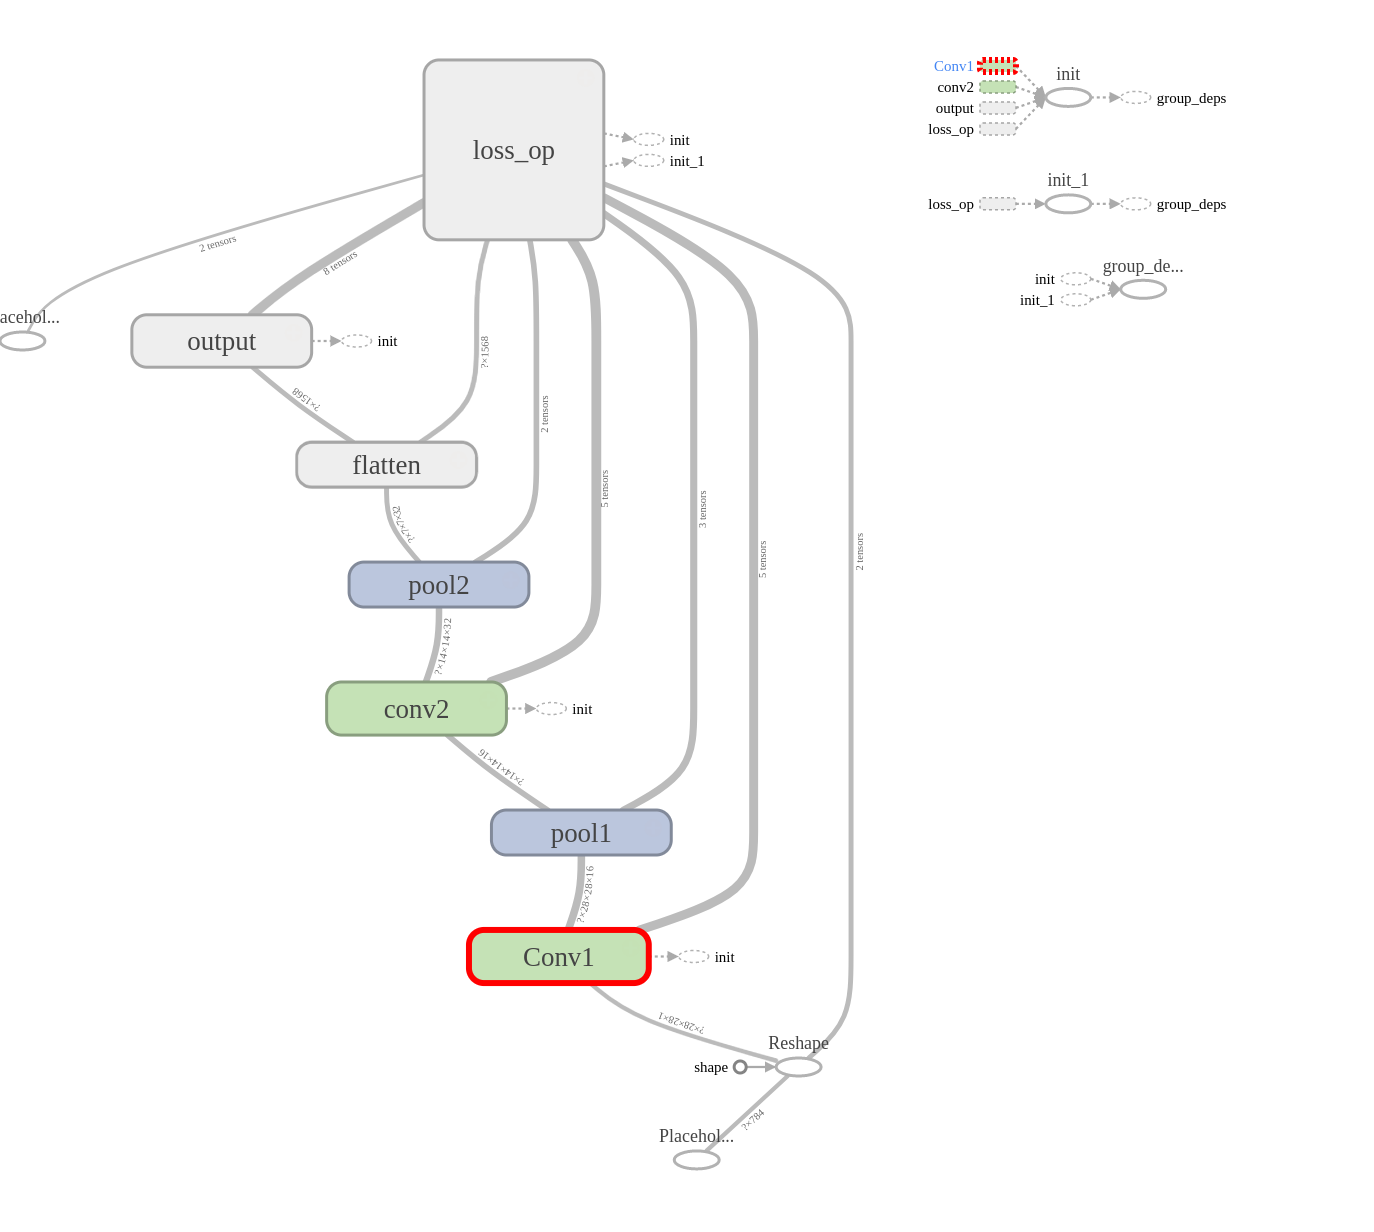
\includegraphics[scale=0.3]{mnist_cnn.png}
\end{figure}
\subsection{用多图编程}
注意当训练一个模型的时候,通常的使用你的代码的方式是用一个图训练你的模型,另一个图评估或者在你的训练好的模型执行推理。在一些情况下,推理图将不同于训练图,例如像dropout,batch normalization在不同的情况下用不同的操作。更进一步,默认的程序像tf.train.Saver用tf.Variable对象的名字在不同的checkpoint中的变量中识别。当用这种方式编程的时候,你可以完全用Python处理建立,执行图,你也可以在同一进程用多个图。TensorFlow提供了一个默认的图隐含的在相同的上下文环境传递所有的API函数。对于一些程序,单个图是足够的,然而tensorFlow也提供了方法操作默认的节点,下面的情况下可能很有用:
\begin{itemize}
	\item 一个tf.Graph为tf.Operation对象定义了tf.Operation的namespace,每个图中的操作必须有独一无二的名字。TensorFlow将通过添加"\_1","\_2"形成独一无二的名字,因此如果它们的名字已经被传出去了,用多个操作创建图给你对操作的名字更好的控制。
	\item 默认的图存储关于每个tf.Operation和tf.Tensor的信息。如果你的程序创建了很多互不连接的子图,用不同的tf.Graph建立子图可能更高效,因此不相关的状态可能被垃圾收集器收集。
\end{itemize}
你可以安装一个不同的tf.Graph作为默认的图,用tf.Graph.as\_default上下文管理器:
\begin{python}
g_1 = tf.Graph()
with g_1.as_default():
    c = tf.constant("Node in g_1")
    sess_1 = tf.Session()
g_2 = tf.Graph()
with g_2.as_default():
    d = tf.constant("Node in g_2")
sess_2 = tf.Session(graph=g_2)
assert c.graph is g_1
assert sess_1.graph is g_1
assert d.graph is g_2
assert sess_2.graph is g_2
\end{python}
查看当前默认的图可以使用tf.get\_default\_graph返回一个tf.Graph对象。
\begin{python}
# Print all of the operations in the default graph.
g = tf.get_default_graph()
print(g.get_operations())
\end{python}
\section{数据集}
Dataset模块允许你从简单的,可重用的片段输入pipeline。例如图像模块的pipeline
也许集合分布式文件系统的数据,随机扰动每张图片,随机融合选中的图片为一个batch来训练,pipeline的text模型能利用元素提取的文本数据,转换它们为查找表embedding的标志符将不同长度的序列放在一起成为一个batch。Dataset API使得处理大型数据,不同数据格式和复杂的转换变得很容易。
一个 Dataset
 API包含两个TebsorFlow抽象。
\begin{itemize}
\item 一个tf.contrib.data.Dataset代表一个元素序列,其中的每个元素代表了一个或者更多的Tensor对象。例如在图像pipeline,一个元素可能是单个的训练样本(一对代表了label和图像数据的tensor)有两种方法创建数据集:
	\begin{enumerate}
		\item 创建一个源(Dataset.from\_tensor\_slices())从一个或者更多的tf.Tensor图像构造数据集。
		\item 应用转换格式从一个或者更多的tf.contrib.data.Dataset对象构造数据集。
	\end{enumerate}
	\item tf.contrib.data.Iterator提供主要的从数据集提取元素的方法当Iterator.get\_next()操作执行的时候从Dataset生成下一个元素,典型的行为作为输入pipeline和你的模型之间的接口。最简单的迭代器(iterator)是"one-shot iterator"它结合了数据集和迭代。用Iterator.initializer操作用不同的数据集重新初始化和参数化一个迭代器,例如在一个程序多次迭代训练样本和验证集。
\end{itemize}
\subsection{基本的机制}
为了开始一个输入pipeline你需要定义一个源。例如从内存中的一些tensor构造一个数据集。你可以使用tf.contrib.data.Dataset.from\_tensors()或者tf.contrib.data.Dataset.from
\newline \_tensor\_slices()。如果你的输入数据在磁盘上,推荐你用TFRecord
格式,你可以构造一个tf.contrib.data.TFRecordDataset。

当你有一个Dataset对象的时候,你可以通过链式方法调用tf.contrib.data.Dataset对象转化成新的Dataset。例如你可以用之前的元素转换作为Dataset.map()(应用一个函数到每个元素)多元素转换像Dataset.batch()。查看文档\href{https://www.tensorflow.org/api_docs/python/tf/contrib/data/Dataset}{tf.contrib.data.Dataset}完成列表转换。
最常用的方法是消耗从Dataset来的值创建一个迭代器对象,提供访问一个元素的数据集的元素一次(调用Dataset.make\_one\_shot\_iterator()),一个tf.contrib.data.Iterator提供两个操作:Iterator.initializer重新初始化你的迭代器状态;Iterator.get\_next()返回迭代器下一个元素的Tensor。
\subsection{数据结构}
一个数据集包含有相同结构的元素。一个元素包含一个或者更多称为组件的tf.Tensor对象。每个组件有tf.DType代表在tensor中元素的数据类型,Dataset.output\_types和Dataset.output\_shapes属性允许你查看每个数据集元素的组件的类型和形状。这些参数的嵌套结构映射元素的结构(也许是一个tensor,一个tensor元组,或者嵌套的tensor元组)
\begin{python}
dataset1 = tf.contrib.data.Dataset.from_tensor_slices(tf.random_uniform([4,10]))
print(dataset1.output_types)#tf.float32
print(dataset1.output_shapes)#(10,)
dataset2 = tf.contrib.data.Dataset.from_tensor_slices((tf.random_uniform([4]))
tf.random_uniform([4,100],maxval=100,dtype=tf.int32))
print(dataset2.output_types)#(tf.float32,tf.int32)
print(dataset2.output_shapes)#((),(100,))
datasets = tf.contrib.data.Dataset.zip((dataset1,dataset2))
print(dataset3.output_types)#(tf.float32,(tf.float32,tf.int32))
print(dataset3.output_shapes)#(10,((),(100,)))
\end{python}
给每个元素的组成命名是很方便的,例如它们代表不同训练样本的特征。另外,你可以用collections.namedtuple或者一个字典映射字符串到tensor代表Dataset的单个元素。
\begin{python}
dataset = tf.contrib.data.Dataset.from_tensor_slices({
	"a":tf.random_uniform([4]),
	"b":tf.random_uniform([4,100],maxval=100,dtype=tf.int32}))
print(dataset.output_types())#{'a':tf.float32,'b':tf.int32}
print(dataset.output_shape)#{'a':(),'b':(100,)}
\end{python}
Dataset转换支持任何的数据结构,当你用Dataset.map(),Dataset.flat\_map和Dataset.filter()转换应用函数到每个元素,元素结构决定函数的参数:
\begin{python}
dataset1 = dataset1.map(lambda x: ...)
dataset2 = dataset2.flat_map(lambda x, y: ...)
# Note: Argument destructuring is not available in Python 3.
dataset3 = dataset3.filter(lambda x, (y, z): ...)
\end{python}
\subsection{创建一个迭代器}
当你创建一个Dataset代表你的输入数据的时候,下一步是创建一个迭代器从数据集中访问元素,Dataset API当前支持一下迭代器:
\begin{itemize}
	\item one-shot
	\item initilizable
	\item reinitilizable
	\item feedable
\end{itemize}
one-shot迭代器是迭代器中最简单的形式,支持在数据集上迭代一次,不需要初始化。One-shot处理大多数的基于队列的输入pipeline,但是它们不支持参数化。用Dataset.range()作为例子:
\begin{python}
dataset = tf.contrib.data.Dataset.range(100)
iterator = dataset.make_one_shot_iterator()
next_element = iterator.get_next()
for i in range(10):
    value = sess.run(next_element)
    assert i == value
\end{python}
initializable迭代器要求你使用前明确的运行iterator.initializer操作。为此它允许你送入一个或者更多的tf.placeholder() tensor\textcolor{red}{初始化你的迭代器},继续用Dataset.range():
\begin{python}
#Base environ pass
max_value = tf.placeholder(tf.int64, shape=[])
dataset = tf.contrib.data.Dataset.range(max_value)
iterator = dataset.make_initializable_iterator()
next_element = iterator.get_next()
sess = tf.Session()
# Initialize an iterator over a dataset with 10 elements.
sess.run(iterator.initializer, feed_dict={max_value: 10})
for i in range(10):
    value = sess.run(next_element)
    assert i == value
# Initialize the same iterator over a dataset with 100 elements.
sess.run(iterator.initializer, feed_dict={max_value: 100})
for i in range(100):
    value = sess.run(next_element)
    assert i == value
\end{python}
一个reinitializable迭代器可以通过多个不同的Dataset对象初始化。例如你也许有一个用随机扰动输入图像提高泛化性的输入pipeline一个验证输入pipeline在没有修改的数据上评价预测。这些pipeline将用于相同结构(每个组件有相同的类型和兼容的形状)的不同的Dataset对象
\begin{python}
# Define training and validation datasets with the same structure.
training_dataset = tf.contrib.data.Dataset.range(100).map(
    lambda x: x + tf.random_uniform([], -10, 10, tf.int64))
validation_dataset = tf.contrib.data.Dataset.range(50)
# A reinitializable iterator is defined by its structure. We could use the
# `output\_types` and `output\_shapes` properties of either `training\_dataset`
# or `validation\_dataset` here, because they are compatible.
iterator = Iterator.from_structure(training_dataset.output_types,
training_dataset.output_shapes)
next_element = iterator.get_next()
training_init_op = iterator.make_initializer(training_dataset)
validation_init_op = iterator.make_initializer(validation_dataset)
# Run 20 epochs in which the training dataset is traversed, followed by the
# validation dataset.
for _ in range(20):
# Initialize an iterator over the training dataset.
    sess.run(training_init_op)
    for _ in range(100):
        sess.run(next_element)
    # Initialize an iterator over the validation dataset.
    sess.run(validation_init_op)
    for _ in range(50):
        sess.run(next_element)
\end{python}
一个feedable迭代器可以和tf.placeholder用在一起来调用tf.Session.run时选择什么通过deed\_dict机制。它提供相同的函数作为重新初始化迭代器,但是当你在不同数据集切换的时候不要求你从数据集开始初始化。例如用相同的训练验证样本你可以用tf.contrib.data.Iterator.from\_string\_handle定义一个feedable迭代器允许你在不同的数据集之间切换:
\begin{python}
# Define training and validation datasets with the same structure.
training_dataset = tf.contrib.data.Dataset.range(100).map(
    lambda x: x + tf.random_uniform([], -10, 10, tf.int64)).repeat()
validation_dataset = tf.contrib.data.Dataset.range(50)
# A feedable iterator is defined by a handle placeholder and its structure. We
# could use the `output\_types` and `output\_shapes` properties of either
# `training\_dataset` or `validation\_dataset` here, because they have
# identical structure.
handle = tf.placeholder(tf.string, shape=[])
iterator = tf.contrib.data.Iterator.from_string_handle(
        handle, training_dataset.output_types, training_dataset.output_shapes)
next_element = iterator.get_next()
# You can use feedable iterators with a variety of different kinds of iterator
# (such as one-shot and initializable iterators).
training_iterator = training_dataset.make_one_shot_iterator()
validation_iterator = validation_dataset.make_initializable_iterator()
# The `Iterator.string\_handle()` method returns a tensor that can be evaluated
# and used to feed the `handle` placeholder.
training_handle = sess.run(training_iterator.string_handle())
validation_handle = sess.run(validation_iterator.string_handle())
# Loop forever, alternating between training and validation.
while True:
# Run 200 steps using the training dataset. Note that the training dataset is
# infinite, and we resume from where we left off in the previous `while` loop
# iteration.
    for _ in range(200):
        sess.run(next_element, feed_dict={handle: training_handle})
    # Run one pass over the validation dataset.
    sess.run(validation_iterator.initializer)
    for _ in range(50):
        sess.run(next_element, feed_dict={handle: validation_handle})
\end{python}
\subsection{消耗迭代器的值}
Iterator.get\_next()方法返回一个或多个迭代器的下一个元素tf.Tensor对象。每次迭代器被计算的时候它们得到数据集中的下一个元素,在TensorFlow中调用Iterator.get\_next()不会立即前进迭代器。相反你需要在一个TensorFlow表达式返回tf.Tensor对象,传递表达式的结果给tf.Session.run得到表达式的结果和下一个迭代器。
如果迭代器到大数据的尾部,执行Iterator.get\_next()操作将报出tf.errors.OutOfRangeError。这个点后迭代器将进入不稳定状态,你必须再次初始化它:
\begin{python}
dataset = tf.contrib.data.Dataset.range(5)
iterator = dataset.make_initializable_iterator()
next_element = iterator.get_next()
# Typically `result` will be the output of a model, or an optimizer's
# training operation.
result = tf.add(next_element, next_element)
sess.run(iterator.initializer)
print(sess.run(result))  # ==> "0"
print(sess.run(result))  # ==> "2"
print(sess.run(result))  # ==> "4"
print(sess.run(result))  # ==> "6"
print(sess.run(result))  # ==> "8"
try:
    sess.run(result)
except tf.errors.OutOfRangeError:
    print("End of dataset")  # ==> "End of dataset"
\end{python}
一个常用的模板是创建一个try-except块的训练循环包装器:
\begin{python}
sess.run(iterator.initializer)
while True:
    try:
        sess.run(result)
    except tf.errors.OutOfRangeError:
        break
\end{python}
如果数据集中的每个元素都有迭代的结构在相同的迭代结果下Iterator.get\_next()将返回一个或者更多的tf.Tensor。
\begin{python}
dataset1 = tf.contrib.data.Dataset.from_tensor_slices(tf.random_uniform([4, 10]))
dataset2 = tf.contrib.data.Dataset.from_tensor_slices((tf.random_uniform([4]), tf.random_uniform([4, 100])))
dataset3 = tf.contrib.data.Dataset.zip((dataset1, dataset2))
iterator = dataset3.make_initializable_iterator()
sess.run(iterator.initializer)
next1, (next2, next3) = iterator.get_next()
\end{python}
注意计算任何next1,next2或者next3将对所有的组件前进迭代器。一个典型的消耗迭代器将不能包含在单个表达式中的所有组件。
\subsection{读输入数据}
\subsubsection{消耗NumPy数据}
如果你的所有数据都适合于存储,一个简单的方法是用Dataset.from\_tensor\_slices()转换它们为tf.Tensor对象创建一个Dataset。
\begin{python}
# Load the training data into two NumPy arrays, for example using `np.load()`.
with np.load("/var/data/training_data.npy") as data:
    features = data["features"]
    labels = data["labels"]
# Assume that each row of `features` corresponds to the same row as `labels`.
assert features.shape[0] == labels.shape[0]
dataset = tf.contrib.data.Dataset.from_tensor_slices((features, labels))
\end{python}
注意上面的代码将在你的TensorFlow图中创建一个嵌入的features和labels作为一个tf.constant()操作。对于小的数据集这是很有用的,但是比较浪费存储,因为数据的内容将被多次复制可能达到tf.GraphDef protocal buffer的2GB限制。
\begin{python}
# Load the training data into two NumPy arrays, for example using `np.load()`.
with np.load("/var/data/training_data.npy") as data:
    features = data["features"]
    labels = data["labels"]
    # Assume that each row of `features` corresponds to the same row as `labels`.
assert features.shape[0] == labels.shape[0]
features_placeholder = tf.placeholder(features.dtype, features.shape)
labels_placeholder = tf.placeholder(labels.dtype, labels.shape)
dataset = tf.contrib.data.Dataset.from_tensor_slices((features_placeholder, labels_placeholder))
# [Other transformations on `dataset`...]
dataset = ...
iterator = dataset.make_initializable_iterator()
sess.run(iterator.initializer, feed_dict={features_placeholder: features,
                                        labels_placeholder: labels})
\end{python}
\subsection{消耗TFRecord数据}
一些数据集有一个或者多个文件。tf.contrib.data.TextLineDataset提供了一个简单的方法从一个或者更多text文件提取
行给定一个或者更多的文件名TextLineDataset将产生一个或者更多的字符串值元素。像TFRecordDataset,TextLineDataset接受filenames作为一个tf.Tensor,因此你可以通过tf.placeholder参数化它
\begin{python}
filenames = ["/var/data/file1.txt", "/var/data/file2.txt"]
dataset = tf.contrib.data.TextLineDataset(filenames)
\end{python}
默认情况下一个TextLineDataset产生文件的每一行,这也许并不是你想要的,例如一个文件的开头行有一些注释。这些行可以用Dataset.skip()移除和Dataset.filter()转换。为了在分割的文件应用这些转换,我们用Dataset.flat\_map()为每个文件创建一个迭代的Dataset
\lstinputlisting[language=Python]{./code/read_data.py}
\subsection{用Dataset.map()处理数据}
Dataset.map(f)通过使用函数f作用于输入数据集的每个元素生成一个新的数据集。它通过函数编程语言用map函数应用到列表。这个函数f接受tf.tensor对象代表一个单个的输入元素,返回一个代表一个数据集中单个元素tf.Tensor对象。它通过标准的TensorFlow操作转化一个元素为另一个。
\subsection{解析tf.Example protocal buffer消息}
一些输入的pipeline从TFRecord格式的文件提取tf.train.Example protocal buffer消息,用tf.python\_io.TFRecordWriter。每个tf.train.Example记录包含一个或者多个特征,输入pipline通常转换这些特征为tensor。
\begin{python}
# Transforms a scalar string `example\_proto` into a pair of a scalar string and
# a scalar integer, representing an image and its label, respectively.
def _parse_function(example_proto):
    features = {"image": tf.FixedLenFeature((), tf.string, default_value=""),
                "label": tf.FixedLenFeature((), tf.int32, default_value=0)}
    parsed_features = tf.parse_single_example(example_proto, features)
    return parsed_features["image"], parsed_features["label"]

# Creates a dataset that reads all of the examples from two files, and extracts
# the image and label features.
filenames = ["/var/data/file1.tfrecord", "/var/data/file2.tfrecord"]
dataset = tf.contrib.data.TFRecordDataset(filenames)
dataset = dataset.map(_parse_function)
\end{python}
\subsection{解码图像数据变换大小}
当在一个真实世界的图像数据中训练一个神经网络,需要转换不同大小到一个同样的大小,因此它们也许处理为一个固定的尺寸
\begin{python}
# Reads an image from a file, decodes it into a dense tensor, and resizes it
# to a fixed shape.
def _parse_function(filename, label):
    image_string = tf.read_file(filename)
    image_decoded = tf.image.decode_image(image_string)
    image_resized = tf.image.resize_images(image_decoded, [28, 28])
    return image_resized, label

# A vector of filenames.
filenames = tf.constant(["/var/data/image1.jpg", "/var/data/image2.jpg", ...])

# `labels[i]` is the label for the image in filenames[i]
labels = tf.constant([0, 37, ...])
dataset = tf.contrib.data.Dataset.from_tensor_slices((filenames, labels))
dataset = dataset.map(_parse_function)
\end{python}
\subsection{用专门的Python logic}
考虑到性能要求,我们鼓励你尽可能用TensorFlow操作处理你的数据。然而当解析你的数据时有是有调用额外的python操作处理数据是有用的。为了这么做,在Dataset.map()转换中调用tf.py\_func()操作
\begin{python}
import cv2

# Use a custom OpenCV function to read the image, instead of the standard
# TensorFlow `tf.read\_file()` operation.
def _read_py_function(filename, label):
  image_decoded = cv2.imread(image_string, cv2.IMREAD_GRAYSCALE)
  return image_decoded, label

# Use standard TensorFlow operations to resize the image to a fixed shape.
def _resize_function(image_decoded, label):
  image_decoded.set_shape([None, None, None])
  image_resized = tf.image.resize_images(image_decoded, [28, 28])
  return image_resized, label

filenames = ["/var/data/image1.jpg", "/var/data/image2.jpg", ...]
labels = [0, 37, 29, 1, ...]

dataset = tf.contrib.data.Dataset.from_tensor_slices((filenames, labels))
dataset = dataset.map(
    lambda filename, label: tf.py_func(
        _read_py_function, [filename, label], [tf.uint8, label.dtype]))
dataset = dataset.map(_resize_function)
\end{python}
\subsection{简单的批处理}
一个最简单的批处理是堆叠数据集中n个连续的元素。Dataset.batch()变换就是这么做的,和tf.stack()一样应用元素的每个组件,每个组件i所有的元素必须有一个相同的形状tensor。
\begin{python}
inc_dataset = tf.contrib.data.Dataset.range(100)
dec_dataset = tf.contrib.data.Dataset.range(0, -100, -1)
dataset = tf.contrib.data.Dataset.zip((inc_dataset, dec_dataset))
batched_dataset = dataset.batch(4)

iterator = batched_dataset.make_one_shot_iterator()
next_element = iterator.get_next()

print(sess.run(next_element))  # ==> ([0, 1, 2,   3],   [ 0, -1,  -2,  -3])
print(sess.run(next_element))  # ==> ([4, 5, 6,   7],   [-4, -5,  -6,  -7])
print(sess.run(next_element))  # ==> ([8, 9, 10, 11],   [-8, -9, -10, -11])
\end{python}
\subsection{批量的tensorpadding}
上面的方法要要求所有的元素有相同的尺寸,然而一些模型(sequence模型)中输入数据有不同的形状。为了处理这些情况,Dataset.padded\_batch()使你通过指定一个或者更多维(需要padding)转换不同形状的tensor为一个batch。
\begin{python}
dataset = tf.contrib.data.Dataset.range(100)
dataset = dataset.map(lambda x: tf.fill([tf.cast(x, tf.int32)], x))
dataset = dataset.padded_batch(4, padded_shapes=[None])

iterator = dataset.make_one_shot_iterator()
next_element = iterator.get_next()

print(sess.run(next_element))  # ==> [[0, 0, 0], [1, 0, 0], [2, 2, 0], [3, 3, 3]]
print(sess.run(next_element))  # ==> [[4, 4, 4, 4, 0, 0, 0],
                               #      [5, 5, 5, 5, 5, 0, 0],
                               #      [6, 6, 6, 6, 6, 6, 0],
                               #      [7, 7, 7, 7, 7, 7, 7]]
\end{python}
Dataset.padded\_batch()转换允许你为每组件的一维度设置不同的pading,它也许有变化的长度或者固定的长度,它可以覆盖padding的值(默认为0)。
\subsection{处理多epoch}
Dataset API提供了两个主要的方法处理相同数据的多个epochs,最简单的方法是用Dataset.repeat()变换数据集在多个epoch、例如,在输入中创建一个数据集10 epochs
\begin{python}
filenames = ["/var/data/file1.tfrecord", "/var/data/file2.tfrecord"]
dataset = tf.contrib.data.TFRecordDataset(filenames)
dataset = dataset.map(...)
dataset = dataset.repeat(10)
dataset = dataset.batch(32)
\end{python}
使用Dataset.repeat()变换没有参数重复输入将不确定。Dataset.repeat()变换连接它的参数每个epochs没有任何结束信号和下一个epoch的开始信号。如果你想接收每个epoch信号,你可以写一个循环在数据集的末尾捕获tf.errors.OutOgRange。
\begin{python}
filenames = ["/var/data/file1.tfrecord", "/var/data/file2.tfrecord"]
dataset = tf.contrib.data.TFRecordDataset(filenames)
dataset = dataset.map(...)
dataset = dataset.batch(32)
iterator = dataset.make_initializable_iterator()
next_element = iterator.get_next()

# Compute for 100 epochs.
for _ in range(100):
    sess.run(iterator.initializer)
    while True:
    try:
        sess.run(next_element)
    except tf.errors.OutOfRangeError:
        break

  # [Perform end-of-epoch calculations here.]
\end{python}
\subsection{随机打乱输入数据}
Dataset.shuffle()用和tf.RandomShuffleQueue方法随即打乱输入数据集,它保持一个固定的buffer平均的从bugger选择下一个元素(查看完整例子):
\begin{python}
filenames = ["/var/data/file1.tfrecord", "/var/data/file2.tfrecord"]
dataset = tf.contrib.data.TFRecordDataset(filenames)
dataset = dataset.map(...)
dataset = dataset.shuffle(buffer_size=10000)
dataset = dataset.batch(32)
dataset = dataset.repeat()
\end{python}
\subsection{用高级APIs}
tf.train.MonitoredTrainingSession API简化了一些在分布式方面运行方面的设置。MonidotedTrainingSession用tf.errors.outOfRangeError作为训练完成的标记,因此用Dataset API,我们推荐用Dataset.make\_one\_shot\_iterator()例如:
\begin{python}
filenames = ["/var/data/file1.tfrecord", "/var/data/file2.tfrecord"]
dataset = tf.contrib.data.TFRecordDataset(filenames)
dataset = dataset.map(...)
dataset = dataset.shuffle(buffer_size=10000)
dataset = dataset.batch(32)
dataset = dataset.repeat(num_epochs)
iterator = dataset.make_one_shot_iterator()

next_example, next_label = iterator.get_next()
loss = model_function(next_example, next_label)

training_op = tf.train.AdagradOptimizer(...).minimize(loss)

with tf.train.MonitoredTrainingSession(...) as sess:
    while not sess.should_stop():
        sess.run(training_op)
\end{python}
为了在tf.estimator.Estimator的input\_fn中使用一个Dataset,我们推荐用Dataset.make\_one\_shot\_iterator(),例如:
\begin{python}
def dataset_input_fn():
    filenames = ["/var/data/file1.tfrecord", "/var/data/file2.tfrecord"]
    dataset = tf.contrib.data.TFRecordDataset(filenames)

# Use `tf.parse\_single\_example()` to extract data from a `tf.Example`
# protocol buffer, and perform any additional per-record preprocessing.
    def parser(record):
        keys_to_features = {
            "image_data": tf.FixedLenFeature((), tf.string, default_value=""),
            "date_time": tf.FixedLenFeature((), tf.int64, default_value=""),
            "label": tf.FixedLenFeature((), tf.int64,
                                    default_value=tf.zeros([], dtype=tf.int64)),
    }
        parsed = tf.parse_single_example(record, keys_to_features)

        # Perform additional preprocessing on the parsed data.
        image = tf.decode_jpeg(parsed["image_data"])
        image = tf.reshape(image, [299, 299, 1])
        label = tf.cast(parsed["label"], tf.int32)

        return {"image_data": image, "date_time": parsed["date_time"]}, label

  # Use `Dataset.map()` to build a pair of a feature dictionary and a label 
  # tensor for each example.
  dataset = dataset.map(parser)
  dataset = dataset.shuffle(buffer_size=10000)
  dataset = dataset.batch(32)
  dataset = dataset.repeat(num_epochs)
  iterator = dataset.make_one_shot_iterator()

  # `features` is a dictionary in which each value is a batch of values for
  # that feature; `labels` is a batch of labels.
  features, labels = iterator.get_next()
  return features, labels
\end{python}
\section{线程和队列}
\begin{quote}
	\emph{注意在TensorFlow1.2之前我们推荐用多线程,队列输入pipeline,在TensorFlow1.2开始我们推荐使用tf.contrib.data模块。tf.contrib.data提供了一个更加简单的结构构建高效的输入pipeline,我们已经停止了之前正在开发的多线程和队列输入pipeline,我们帮依然维护旧的代码的开发者维护文档。}
\end{quote}
%多线程及时是一个强有力的而且广泛使用的支持一步计算的机制,入上面章节所述,TensorFlow计算图节点和计算图实现,一个队列是一个已经准备好的节点,向一个变量;以它节点可以修改它的内容。类似的,节点可以入队新的元素到队列或者从队列中出去已近存在的元素,TensorFlow队列提供了一个方法结合多个计算步。如果队列为空依然出队或者队列已满依然入队豆浆产生阻塞,挡这两个条件不满足的时候阻塞解除基础处理。TensorFlow实现了多个队列类,不同的类之间的不同是元素从队列移除的顺序。为了更好的理解我们考虑一个简单的情况我们创建"First in first out"队列然后填充0.然后我们构造一张图从队列中获取元素增加1,然后将它放在队列的尾部,慢慢地队列中的数字增加。
\begin{python}
sess = tf.Session()
q = tf.FIFOQueue(3,"float")
init = q.enqueue_many(([0.,0.,0.],))
x = q.dequeue()
y = x+1
q_inc = q.enqueue([y])
init.run(session=sess)
q_inc.run(session=sess)
q_inc.run(session=sess)
q_inc.run(session=sess)
q_inc.run(session=sess)
\end{python}
Enqueue,EnqueueMany和Dequeue是一个特别的节点。它们是指向队列真实值的指针,允许它们改变状态。我们推荐你考虑这些操作的时候用面向对象的理解,事实上在Python API中这些操作通过调用队列的方法。
\begin{quote}
	\emph{注意Queue方法必须运行在相同的设备上,不兼容的设备放置将在创建这些操作的时候被忽略}
\end{quote}
\subsection{队列用法}
像tf.FIFOQueue和tf.RandomShuffleQueue是在图上执行异步计算的重要的TensorFlow对象。典型的队列输入pipline用RandomShuffleQueue为训练模型准备输入:
\begin{itemize}
	\item 多线程准备训练数据和将数据入队
	\item 训练线程执行训练操作从队列出队mini-batch
\end{itemize}
我们推荐使用Dataset的shuffle和batch方法完成这个任务。然而,如果你仍然愿意使用队列版本,你可以在tf.train.shuffle\_batch中找到完美的实现。

下面展示一个简单的实现,这个函数获取一个source tensor,capacity和batch size作为参数返回一个批量打乱的出队tensor。
\begin{python}
def simple_shuffle_batch(source, capacity, batch_size=10):
  # Create a random shuffle queue.
    queue = tf.RandomShuffleQueue(capacity=capacity,
                                  min_after_dequeue=int(0.9*capacity),
                                  shapes=source.shape, dtypes=source.dtype)

    # Create an op to enqueue one item.
    enqueue = queue.enqueue(source)

    # Create a queue runner that, when started, will launch 4 threads applying
    # that enqueue op.
    num_threads = 4
    qr = tf.train.QueueRunner(queue, [enqueue] * num_threads)

    # Register the queue runner so it can be found and started by
    # `tf.train.start\_queue\_runners` later (the threads are not launched yet).
    tf.train.add_queue_runner(qr)

    # Create an op to dequeue a batch
    return queue.dequeue_many(batch_size)
\end{python}
当tf.train.start\_queue\_runners开始的时候,或者直接通过tf.train.MonitoredSession,QueueRunner将在后台开启进程填充队列,同时主线程执行dequeue\_many操作从中拉取数据,现在这些操作不相互依赖,除非间接地通过队列的内部依赖。简单的用这个函数像这样:
\begin{python}
# create a dataset that counts from 0 to 99
input = tf.constant(list(range(100)))
input = tf.contrib.data.Dataset.from_tensor_slices(input)
input = input.make_one_shot_iterator().get_next()

# Create a slightly shuffled batch from the sorted elements
get_batch = simple_shuffle_batch(input, capacity=20)

# `MonitoredSession` will start and manage the `QueueRunner` threads.
with tf.train.MonitoredSession() as sess:
    # Since the `QueueRunners` have been started, data is available in the
    # queue, so the `sess.run(get\_batch)` call will not hang.
    while not sess.should_stop():
        print(sess.run(get_batch))
\end{python}
输出
\begin{python}
[ 8 10  7  5  4 13 15 14 25  0]
[23 29 28 31 33 18 19 11 34 27]
[12 21 37 39 35 22 44 36 20 46]
\end{python}
对于更多的情况有tf.train.MonitoredSession提供的自动线程启动和管理是足够的,在极少的情况下不行,TensorFlow提供了手动管理你的线程的工具。
\subsection{手动线程管理}
正如我们看到的,TensorFlow Session是多线程的而且是线程安全的,因此多线程能够容易的在相同的会话和运行操作中使用。然而,不总是很容易实现一个Python程序按照要求驱动线程,所有的线程必须能同时停止,特别是必须捕获和报告,队列停止的时候必须被合适的关闭。TensorFlow提供了两个类:tf.train.Coordinator和tf.train.QueueRunner。这两个类帮助多线程一起停止,向程序报告异常等待它们停止,QueueRunner类被用于创建一个线程协作同一队列中的入队tensor。
\subsection{Coordinator}
tf.train.Coordinator类管理TensorFlow程序的后台线程帮助多线程一起停止,关键的方法是:
\begin{itemize}
	\item tf.train.Coordinator.should\_stop:如果线程应该被停止返回True。
	\item tf.train.Coordinator.request\_stop:请求应该停止的线程。
	\item tf.train.Coordinator.join:等待直到指定的线程被停止。
\end{itemize}
你首先创建一个Coordinator对象然后创建一些用于协调的线程。线程通常循环运行当shold\_stop为True是停止。任何线程都可以决定计算应该被停止。它仅仅必须调用request\_stop(),should\_stop()返回True是其它线程停止。
\begin{python}
# Using Python's threading library.
import threading

# Thread body: loop until the coordinator indicates a stop was requested.
# If some condition becomes true, ask the coordinator to stop.
def MyLoop(coord):
    while not coord.should_stop():
    ...do something...
    if ...some condition...:
        coord.request_stop()

# Main thread: create a coordinator.
coord = tf.train.Coordinator()

# Create 10 threads that run 'MyLoop()'
threads = [threading.Thread(target=MyLoop, args=(coord,)) for i in range(10)]

# Start the threads and wait for all of them to stop.
for t in threads:
  t.start()
coord.join(threads)
\end{python}
显然,coordinator可以管理线程做不同的事。它们不是必须和上面的例子一样。coordinator也支持捕获和报告异常,查看\href{https://www.tensorflow.org/api_docs/python/tf/train/Coordinator}{tf.train.Coordinator}文档查看更多信息。
\subsection{QueueRunner}
tf.train.QueueRunner类创建一些线程重复执行入队操作。这些线程可以用coordinator一起停止,另外一个队列runner将运行一个closer操作,如果在coordinator中的队列被报告异常将关闭队列。你可以用一个队列runner实现下面的架构,首先用一个TensorFlow为输入样本建立一个图,添加操作处理将样本送入队列,添加训练操作从队列出队。
\begin{python}
example = ...ops to create one example...
# Create a queue, and an op that enqueues examples one at a time in the queue.
queue = tf.RandomShuffleQueue(...)
enqueue_op = queue.enqueue(example)
# Create a training graph that starts by dequeueing a batch of examples.
inputs = queue.dequeue_many(batch_size)
train_op = ...use 'inputs' to build the training part of the graph...	
\end{python}
在Python的训练程序中,创建一个QueueRunner将运行一些线程处理入队样本、创建一个Coordinator要求queue runner用coordinator开启它的线程。用coordinator写一个训练循环。
\begin{python}
# Create a queue runner that will run 4 threads in parallel to enqueue
# examples.
qr = tf.train.QueueRunner(queue, [enqueue_op] * 4)

# Launch the graph.
sess = tf.Session()
# Create a coordinator, launch the queue runner threads.
coord = tf.train.Coordinator()
enqueue_threads = qr.create_threads(sess, coord=coord, start=True)
# Run the training loop, controlling termination with the coordinator.
for step in range(1000000):
    if coord.should_stop():
        break
    sess.run(train_op)
# When done, ask the threads to stop.
coord.request_stop()
# And wait for them to actually do it.
coord.join(enqueue_threads)
\end{python}
\subsection{处理异常}
线程通过队列runner启动做的比仅仅运行入队操作要多。它们捕获处理队列生成的异常,包括用于报告队列被关闭的tf.errors.OutOfRangeError异常。一个训练中的程序用一个coordinator必须类似的在主循环中捕获和报告异常。下面是上面训练循环的一个改进的例子:
\begin{python}
try:
    for step in range(1000000):
      if coord.should_stop():
        break
      sess.run(train_op)
except Exception, e:
    # Report exceptions to the coordinator.
    coord.request_stop(e)
finally:
    # Terminate as usual. It is safe to call `coord.request\_stop()` twice.
    coord.request_stop()
    coord.join(threads)
\end{python}
\section{embeddings}
一个embedding是一个从离散对象,像字映射为一个真实值的向量,例如一个英文字符的300维的embedding可能包括:
\begin{python}
blue:  (0.01359, 0.00075997, 0.24608, ..., -0.2524, 1.0048, 0.06259)
blues:  (0.01396, 0.11887, -0.48963, ..., 0.033483, -0.10007, 0.1158)
orange:  (-0.24776, -0.12359, 0.20986, ..., 0.079717, 0.23865, -0.014213)
oranges:  (-0.35609, 0.21854, 0.080944, ..., -0.35413, 0.38511, -0.070976)
\end{python}
embedding让你能在离散的数据上应用机器学习,分类器,更常用的神经网络都被设计为一个高密度的连续向量(所有的值都用来定义一个对象)如果离散对象被编码为一个离散的原子,有独一无二的id号,它们阻止学习和泛化,一种考虑embeddings的方法是转化非向量的对象为有用的机器学习输入。,embeding作为机器学习的输出也是有用的,因为embedding映射对象为向量,在向量空间中的应用是类似的。一个通常的用法是找到一个最接近的邻居。用和相面相同的word embedding,例如对于每个字和相关的角度这里有三个接近的邻居:
\begin{python}
blue:  (red, 47.6°), (yellow, 51.9°), (purple, 52.4°)
blues:  (jazz, 53.3°), (folk, 59.1°), (bluegrass, 60.6°)
orange:  (yellow, 53.5°), (colored, 58.0°), (bright, 59.9°)
oranges:  (apples, 45.3°), (lemons, 48.3°), (mangoes, 50.4°)
\end{python}
这将告诉程序苹果和橙子类似度($45.3^o$)比柠檬和橙子($48.3^o$)更类似。
\subsection{训练一个embedding}
为了在TensorFlow中训练word embedding,首先你需要分隔文字成单词赋值给词汇表中的每一个单词一个整数。假设我们已经做了这步,word\_ids是一个整数向量。例如句子"I have a cat."可能被分割成["I","have","a","cat","."]然后相关的word\_ids tensor形状为[5]由5个整数组成。为了得到这些单词ids embeded,我们需要用tf.gather函数按照下面创建embedding变量。
\begin{python}
word_embeddings = tf.get_variable(“word_embeddings”,
    [vocabulary_size, embedding_size])
embedded_word_ids = tf.gather(word_embeddings, word_ids)
\end{python}
在这之后tensor embedded\_word\_ids在我们的例子中将有形状[5,embedding\_size]同时包含5个单词的embeddings(dense vector)。变量word\_embeddings将被学习,在训练结束后它将包含所有在词汇表中的embeddings。embeddings可能被多种方式训练,依靠数据变量。例如可以用循环神经网络从语料中的句子的前一个单词预测下一个单词或者用两个网络做多种语言的翻译。这个方法在\textbf{字词的向量表示}中有描述,但是上面的所有情况下有一个像上面的embedding变量和用tf.gather的embbedded word。
\subsection{可视化Embeddings}
TensorBoard有一个内建的可视化器,称为EmbeddingProjector,用于交互式的embedding可视化。embedding projector将从你的checkpointer文件读取embeddings用PCA映射它们到3维空间。对于PCA的可视化查看\href{http://setosa.io/ev/principal-component-analysis/}{这里},另一个有用的映射是t-SNE。如果你正在embedding上工作,你可能像添加labels/images到数据点。你可以通过生成一个包含每个点的labels和用我们的Python API映射器的配置\href{https://www.tensorflow.org/programmers_guide/embedding#metadata}{metadata file},或者在和你的checkpoint文件相同多个目录手动构造和保存一个projector\_config.pbtxt。
\subsection{创建}
\begin{enumerate}
	\item 设置一个2维tensor保存你的embedding。
		\begin{python}
			embedding_var = tf.get_variable(...)
		\end{python}
	\item 定期保存你模型的变量到LOG\_DIR目录中
		\begin{python}
			saver = tf.train.Saver()
			saver.save(session,os.path.join(LOG_DIR,"model.ckpt"),step)
		\end{python}
	\item 结合meta data和你的embedding(可选)
\end{enumerate}
如果你有任何的metadata(labels,images)结合你的embedding,你可以调用TensorBoard通过指定存储在LOG\_DIR中的一个projector\_config.pbtxt或者用你自己的PythonAPI。例如下面的projector\_config.pbtxt结合word\_embedding tensor和存储在\$LOG\_DIR/metadata.tsv的metadata文件。
\begin{python}
embeddings {
	  tensor_name: 'word_embedding'
	    metadata_path: '$LOG_DIR/metadata.tsv'
	   }
\end{python}
相同的配置可以通过下面的代码段一程序产生:
\begin{python}
from tensorflow.contrib.tensorboard.plugins import projector
# Create randomly initialized embedding weights which will be trained.
vocabulary_size = 10000
embedding_size = 200
embedding_var = tf.get_variable('word_embedding', [vocabulary_size, embedding_size])
# Format: tensorflow/tensorboard/plugins/projector/projector_config.proto
config = projector.ProjectorConfig()
# You can add multiple embeddings. Here we add only one.
embedding = config.embeddings.add()
embedding.tensor_name = embedding_var.name
# Link this tensor to its metadata file (e.g. labels).
embedding.metadata_path = os.path.join(LOG_DIR, 'metadata.tsv')
# Use the same LOG_DIR where you stored your checkpoint.
summary_writer = tf.summary.FileWriter(LOG_DIR)
# The next line writes a projector_config.pbtxt in the LOG_DIR. TensorBoard will
# read this file during startup.
projector.visualize_embeddings(summary_writer, config)
\end{python}
在你运行你的模型和训练你的embedding后,运行TensorBoard和指定job的LOG\_DIR
\begin{python}
tensorboard --logdir=LOG_DIR
\end{python}
点击顶端面板的Embedding选择合适的运行。
\subsection{metdadata}
通常embeddings有metedata结合。metadata应该被存储在和模型的checkpoint分隔的文件中,因此metadata不是可训练的模型的参数。这是应该为\href{https://en.wikipedia.org/wiki/Tab-separated_values}{TSV file}(显示红色标签),第一行十粗体显示的表头和包含metadata值得子序列行。
\begin{lstlisting}{language=Python}
Word\tFrequency
Airplane\t345
Car\t241
...
\end{lstlisting}
有不明确的和主要数据文件的关键共享,而不是在madatada文件中的顺序和embedding tensor里面的顺序相匹配,换句话说第一行是头信息,metadata文件中(i+1)行和存储在checkpoint文件中的embedding tensor的第i行相关。
\begin{quote}
	\emph{如果TSV metadata文件仅仅有一列,我们不需要第一行假设每一行是embedding的label,我们包括这个例外,因为它匹配通常用的"vocab file"格式。}
\end{quote}
\subsection{图像}
如果你有图像和你的embedding结合,你将需要生成一个每个数据点缩略图组成的图像。它被称为\href{https://www.google.com/webhp#q=what+is+a+sprite+image}{sprite image}。sprite应该有和存储进行优先顺序的缩略图相同的行和列:第一个数据点放在是左上角最后一个数据放在右下角。

\begin{tabular}{|c|c|c|}
	\hline
	0&1&2\\
	\hline
	3&4&5\\
	\hline
	6&7&\\
	\hline
\end{tabular}

注意上面例子的最后一个元素不是必须填,对于具体的sprite例子查看10000张手写体数据\href{https://www.tensorflow.org/images/mnist_10k_sprite.png}{sprite image}
\begin{quote}
	\emph{注意我们当前支持$8192px\times8192px$}
\end{quote}
在够早了sprite后你需要告诉Embedding Projector到哪里寻找它:
\begin{python}
embedding.sprite.image_path = PATH_TO_SPRITE_IMAGE
	# Specify the width and height of a single thumbnail.
	embedding.sprite.single_image_dim.extend([w, h])
\end{python}
\subsection{交互}
Embedding Projector有三个面板:
\begin{enumerate}
	\item 左上角的Data面板,你也已选择运行embedding tensor和数据列标上颜色和label points。
	\item 左下角的Projections面板选择projection的类型(PCA,tSNE)
	\item 右边的Insepctor面板,这里你能搜索类似的点查看最近邻居的列表
\end{enumerate}
\subsection{Projections}
Embedding Projector有三种方法减少数据集的维度:两个线性一个非线性。每二个方法可以被用来创建一个二维或者三维视图。

PCA:一个直接的降维技术,Embedding projectorj计算10个主成分。菜单让你映射这些成分为任何二维或者三维。PCA是一个线性projection,检查全局结构时很有效
。

t-SNE:一个流行的非线性降维Embedding Projector提供二维和三维视图。客户端执行算法的每一步都被更新动画。因为t-SNE经常保留一些本地结构,对于本利邻居和发现集群是很有用的。尽管对于高维数据可视化很有用,t-SNE画图可能会有一些神秘或者难以理解,查看\href{http://distill.pub/2016/misread-tsne/}{great artical}查看t-SNE如何高效使用。

Custom:你也可以构造基于文本搜索查找在空间中有用的方向的特别的线性projections。为了定义一个projection轴,输入两个搜索字符串或者正则表达式。程序计算标签和搜索结果配的标签的中心,在不同的向量中心作为一个projection轴。
\subsection{导航}
为了探索数据集,用2维或者3维视图查看,缩放,旋转和用自然的手势点击和拖动面板。点击一个点引起右边面板显示一个确定的最相邻的文本列表。最相邻的点本身在projection被强调。

缩放进入集群给定一些信息,但是有时候更有用的是限制自己点的视角和在这些点上执行projection。,你可以用多种方式选择点:
\begin{enumerate}
	\item 在点击点后,相邻的点也被选中。
	\item 在搜索后匹配的查询被选中。
	\item Embedding选择,点击一个点拖动定义一个选择范围。
\end{enumerate}
在选择一个数据集点后,你可以用右边的inspector面板隔离这些点用isolate Pointes进一步分析,
\begin{figure}[H]
	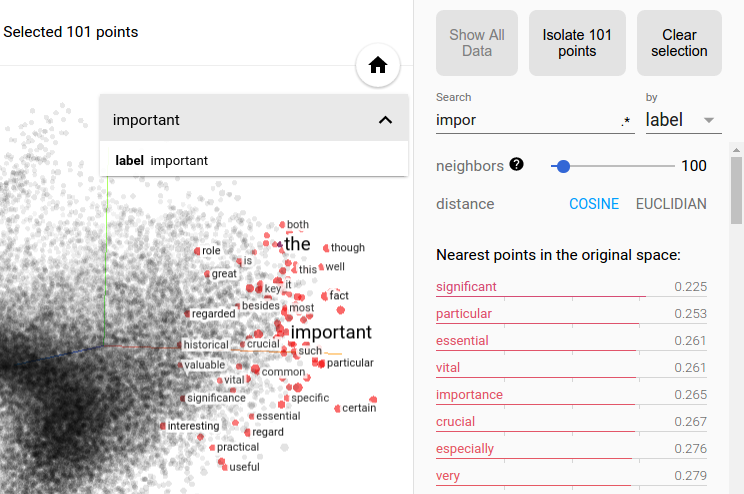
\includegraphics[scale=0.5]{embedding-nearest-points.png}
	\caption{important最相邻的embedding数据集}
\end{figure}
custom projection结合过滤会很有用,下面我们过滤和"politics"100个最相邻的点,project它们在x轴上从好到坏,向量表示,y轴水机。你可以看右边的我们有"ideas","science",\newline "perspective","journalism"左边有"crisis","violence"和"conflict"。
\begin{figure}
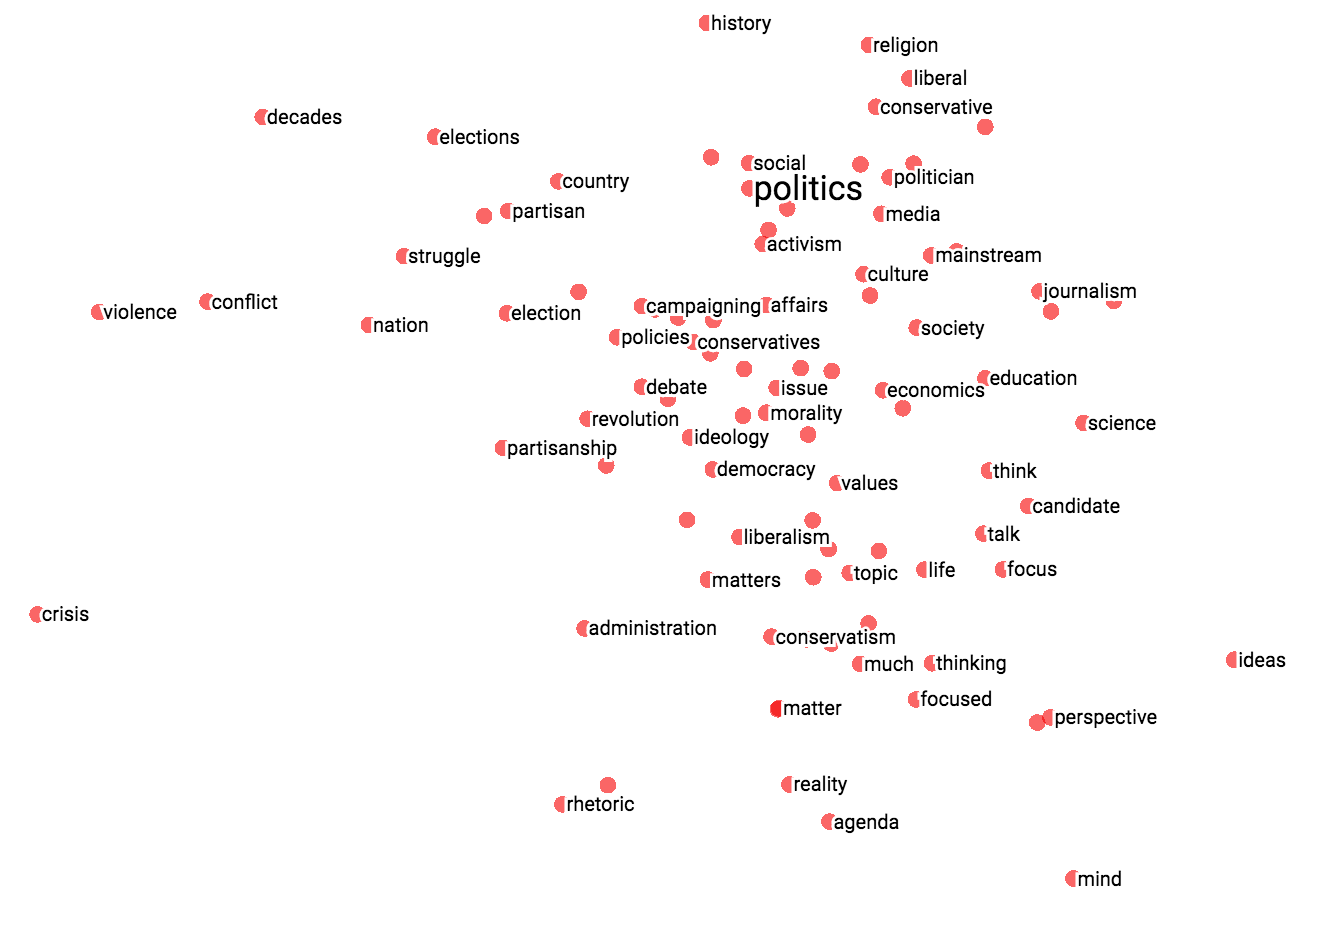
\includegraphics[scale=0.3]{embedding-custom-projection.png}
\end{figure}

\subsection{合作的特性}
为了分享你的发现你可以用右上角的bookmark面板保存当前状态(包括计算任何projection的坐标)为一个小文件。Projector可能被指定到一个或者更多文件,产生下面的面板,其它人可以通过标签序列查看。
\begin{figure}[H]
	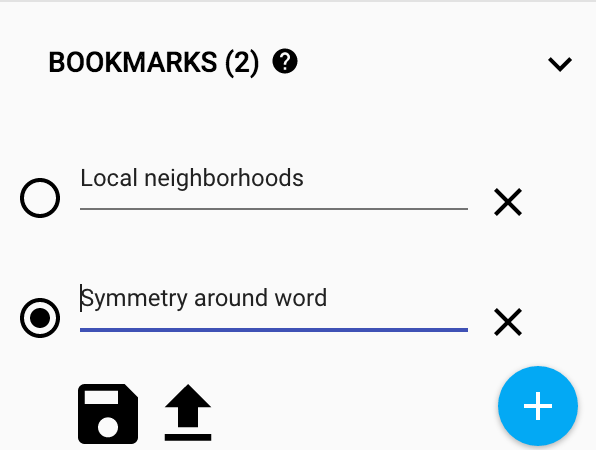
\includegraphics[scale=0.5]{embedding-bookmark.png}
\end{figure}
\subsection{简单的问答}
embedding是一个动作还是一个事物?两者都是,人们谈论向量空间的embedding word形成embedding(事物)。通常两个是一个从离散对象到向量映射embedding概念,创建应用映射是一个行为,但是映射是一个事物。

是高维还是低维embedding?300维的向量字词空间,例如当和上百万的字词空间相比是低维。但是数学上它是高维,显示了大量和人们直觉上的2维或者三维空间不一致的特性。

embedding和embedding layer是一样的吗?不是,一个embedding layer是神经网络的一部分,不是一个embedding是一个更常用的概念。
